\documentclass[11pt,a4paper,twoside,titlepage]{scrbook}
\usepackage[utf8]{inputenc}
\usepackage[ngerman, english]{babel}
\usepackage[pdfborder={0 0 0}]{hyperref}
\usepackage{amsmath}
\usepackage{amsfonts}
\usepackage{amssymb}
\usepackage{graphicx}
\usepackage{geometry}
\usepackage{tikz}
\usepackage{amsthm}
\usepackage{algorithmic}
\usepackage{algorithm}
\usepackage{float}
\usepackage{caption}
\usepackage{subcaption}
\usepackage{mathtools}
\usepackage{float}
\usepackage[section]{placeins}


\clubpenalty=1000
\widowpenalty=1000

\theoremstyle{definition}
\newtheorem{definition}{Definition}[section]
\newtheorem{lemma}{Lemma}
\newtheorem{theorem}{Theorem}
\newtheorem{corollary}{Corollary}




\begin{document}
	
	\frontmatter

	%----- TITLE PAGE -----
	
	\begin{titlepage}
		%\noindent\makebox[\linewidth]{\rule{\paperwidth}{0.4pt}}
	
		\begin{tikzpicture}[remember picture, overlay]
		\node [anchor=north east, inner sep=0pt]  at (17.9,2)%(current page.north east)
			{\includegraphics[height=3.5cm]{figures/tu-bs_logo.jpg}};
		\end{tikzpicture}
		
		\centering
		\vspace{5cm}
		{\scshape\huge Bachelor Thesis\par}
		\vspace{1.5cm}
		{\Huge\bfseries Computing Motion Plans for Assembling Particles with Global Control \par}
		\vspace{3cm}
		{\huge Patrick Blumenberg\par}
		\vfill
		Institut für Betriebssysteme und Rechnerverbund\\
		\vfill
		
		Supervised by\par
		Prof. Dr. Aaron Becker\par
		Dr. Arne Schmidt\par
		
		\vfill
		
		% Bottom of the page
		{\large \today\par}
	\end{titlepage}
	
	\cleardoublepage
	
	% statement of originality
	\thispagestyle{plain} % no header
	\vspace*{7cm}
	\centerline{\bfseries Statement of Originality}
	\vspace*{1em}
	\noindent
	This thesis has been performed independently with the support of my supervisor/s.
	To the best of the author's knowledge, this thesis contains no material previously
	published or written by another person except where due reference is made in the text.
	
	\par
	\bigskip\noindent Braunschweig, \today \par
	\vspace*{10mm}
	\hfill\hrulefill
	\cleardoublepage
	
	
	\chapter*{Aufgabenstellung / Task Description}


\paragraph{Deutsch:}
\begin{otherlanguage}{ngerman}
Wenn es darum geht, Formen im Micro- und Nanobereich zusammenzubauen, ist es aufgrund der Größe der auftretenden Komponenten, begrenzter Rechenleistung und limitierter Energiekapazität sehr schwierig, einzelne Partikel an ihre jeweilig gewünschte Position zu bewegen. Eine Möglichkeit wurde von Erik Winfree 1998 vorgeschlagen, bei der alle (quadratischen) Partikel durch Diffusion aufeinandertreffen und unter verschiedenen Aspekten und Bedingungen aneinander haften bleiben. Eine andere Möglichkeit besteht darin, alle Partikel gleichzeitig durch eine äußere Kraft (zum Beispiel ein Magnetfeld) zu bewegen. In diesem \glqq Tilt-Modell\grqq bewegen sich die Partikel dabei solange in die gewünschte Richtung, bis sie auf ein anderes Partikel oder ein Hindernis treffen. Frühere Arbeiten trafen dabei allerdings oft Annahmen über die Startkonfiguration der Partikel oder verlangte speziell konstruierte Umgebungen. Zum Beispiel können die Partikel in Depots liegen, aus denen die Partikel extrahiert werden können.

Herr Blumenberg soll sich im Rahmen seiner Abschlussarbeit mit dem Konstruieren von Formen im Tilt-Modell beschäftigen, wobei keine Annahmen über die Startkonfiguration getroffen werden sollen. Dabei ist es interessant, wie gut Instanzen in der Praxis gelöst werden können und welche Inputparameter den größten Einfluss auf das Problem haben. Dazu gehört nicht nur das Lösen mit heuristischen Ansätzen, sondern auch das Bestimmen optimaler Bewegungspläne. Eine theoretische Analyse, wie beispielsweise Schranken für die Länge eines Bewegungsplans, ist wünschenswert.
\end{otherlanguage}

\medskip

\paragraph{English:}
When assembling structures at the micro or nanoscale, moving particles to desired target locations is often challenging due to the small size, limited computing power, or limited energy capacity. In 1998, Erik Winfree proposed a model in which all particles move by diffusion and connect if they are compatible. Alternatively, in the “tilt model,” particles are actuated by an external force, e.g., gravitational or magnetic forces. The external force moves all particles in the selected direction unless blocked by another particle or an obstacle. Related work considered the tilt model but often required either the particles to have specific starting conditions such as starting all particles in depots or required specialized workspace configurations designed to make manipulation easier.

In his thesis, Mr. Blumenberg’s task is to design algorithms that assemble structures using the tilt model on randomly generated workspaces with randomly placed starting configurations. One exciting outcome will be studying how good instances can be solved in practice and analyzing which parameters have the most significant effect on the difficulty of the motion planning problem. The task includes heuristics and computing optimal motion plans that minimize the number of steps. Theoretical analysis finding bounds for the length of a motion plan is desired.
	
	
	%---------------------
	\chapter*{Abstract}

In this thesis we developed a heuristic approach for the motion planning problem of assembling structures with magnetic modular cubes, developed and researched by Bhattacharjee et al.\ \cite{Bhattacharjee2022}, in the 2-dimensional special Euclidean group, the space of rigid movements in a 2-dimensional plane.
Magnetic modular cubes are cube-shaped bodies with embedded permanent magnets uniformly controlled by a global time varying magnetic field surrounding the workspace.

A 2D-physics simulator is use to simulate global control and the resulting continuous movement of magnetic modular cube structures as well as magnetic attraction and repulsion, while detecting and resolving collision.
The simulator allows closed-loop control algorithms for planning the connection of two structures at desired faces.
This developed sequences of movements, called local plans, will be used on a global scale to plan the assembly of specified target structures in a rectangular workspace with no internal obstacles.
The assembly is done by generating a set of building instructions for a target structure represented as a graph that we traversed in a depth first search approach with applying local plans to current states of the workspace.

We analyze how target structures of varying sizes and shapes in different rectangular workspaces affect planning time and the rotational-cost of movements.
The traversal of the building instruction graph can be further optimized for which we present three strategies and their effect on the performance of the global planner.
The majority of randomly created instances in our experiments can be solved in under $200$ seconds for structures of up to $12$ cubes, but certain attributes of target structures can decrease efficiency drastically.
	
	\tableofcontents
	
	%% Remove listoffigures or listoftables if not needed!
	\listoffigures
	
	%\listoftables
	
	\mainmatter
	
	\chapter{Introduction}

Self-assembling modular parts forming bigger structures, is a well known concept in nature and most functionalities of living organisms follow this principle \cite{bishop2005}.
Structures can be assembled and disassembled depending on the task they should accomplish during a given point in time. 
Resembling this concept, with self-reconfiguring robot swarms, has promising applications in the Future.
Biomedical applications could be targeted drug delivery or drug screening \cite{sitti2015}, or it could be used for milliscale and microscale manufacturing \cite{pelrine2016}.

Designing robots at these small scales faces serious problems.
Equipping each robot with its own sensors, actuation-system, connection-system and power supply seem very infeasible, in terms of the sheer size and power-limitations \cite{white2007}.
Therefore, the use of external global control, effecting every robot uniformly, seem like a promising solution \cite{white2007}.
Using robots, with no other system than embedded permanent magnets, has all the desired effects.
Robots can be controlled by an external magnetic field and also connect to each other without any internal power supply \cite{saab2019}.

One example for magnetically controlled robots are the magnetic modular cubes by Becker et al. \cite{Becker2022}, which are the subjects of this thesis.
We will develop a simulation, that simulates the behavior of magnetic modular cubes, without assuming discrete movement or limiting the degree of freedom for rotations.
The simulation will be used for developing closed loop planing algorithms, which provide a control sequence to assemble desired target shapes.
For that it is necessary to develop a local planner that is able to connect structures at desired faces.
We will look at the difficulties and problems that occur, when working with magnetic modular cubes in the 2-dimensional special euclidean group.


\section{Related Work}

Motion planning is a crucial subject in the field of robotics.
The goal is to change the initial state of a robot to a desired goal state, by performing actions which the robot is capable of.
The state of the system is also called a configuration and all possible configurations a robot can be in is defined as the configuration-space.
The dimension of the configuration-space gains rapidly in complexity by increasing the number of robots and possible actions.
It is difficult to engineer algorithms that explore these huge configuration-spaces and provide a sequence of actions that lead to the goal configuration, or report failure, if the goal is not reachable.
A lot of research was done on motion planning and the textbooks \cite{LaValle2006} and \cite{Mueller2019} offer a great overview and also explain a lot of important concepts in detail.

When working with configuration-spaces that are uncountable infinite, like the special euclidean group, one of these concepts is sample-based motion planing.
%it is not only impossible to cover the howl space, it is also unclear how to traverse it.
By taking samples, you can reduce the configuration space to a finite object, but you might lose possible solutions.
Algorithms like that are not complete anymore, but by using a good sampling technique you can get arbitrarily close to any point, and therefore these algorithms can be called resolution complete.
Ways of sampling include random sampling or using a grid with a resolution that is dynamically adjustable.
After sampling, conventional discrete planning algorithms can be applied \cite{LaValle2006}.

One state of the art sample-based approach are algorithms that use rapidly-exploring random trees (RRT).
This method tries to move into the direction of a randomly chosen sample from the nearest already explored configuration, that way the space gets explored uniformly without being too fixated on the goal configuration \cite{lavalle1998,lavalle2001}.

When working with multiple robots, the question of how these interact with each other comes to mind.
One interesting idea is that single robots can connect to form bigger structures.
This is referred to as self-assembly and E. Winfree \cite{winfree1998} proposed the abstract Tile Assembly Model (aTAM) in the context of assembling DNA.
In this model, particles can have different sets of glues and connect according to certain rules regarding the glue type.
However, he considers this process as nondeterministic, so there is no exact instruction on how to assemble a desired structure.

One model more related to the here used magnetic modular cubes is the Tilt model from Becker et al. \cite{Becker2014_SP}.
In the Tilt model, all tiles move either one step or the maximum amount, until hitting an obstacle, into one of the cardinal directions.
It offers a solution when robots are controlled uniformly by external global control inputs.
In this paper it is shown, that transforming one configuration into another, known as the reconfiguration-problem, is NP-hard.
Following work \cite{Becker2014} also proves, that finding an optimal control sequence, minimizing the number of actions, for the configuration-problem is PSPACE-complete.
Furthermore, research is done on designing environments in which the Tilt model can be used to accomplish certain tasks.
In particular, Becker et al. \cite{Becker2014} create connected logic gates that can evaluate logical expressions.

More on the side of self-assembly, in \cite{Fekete2020} the construction of desired shapes using the tilt model is researched.
It presents a method that can determine a building sequence for a polyomino by adding one tile at a time, considering the rules of Tilt.
Ways of modifying the environment to create factories constructing shapes in a pipeline by repeating the same global control inputs, are also examined.
Shapes can not only be constructed by adding one tile at a time.
Two multi-tiled shapes can connect to an even bigger structure.
One article considering the construction with so called sub-assemblies is proposed by A. Schmidt \cite{Schmidt2018}.

Most recently, Becker et al. \cite{Becker2022} developed the magnetic modular cubes.
These robots contain embedded permanent magnets and have no computation or power supply.
Therefore, they are all controlled uniformly by an external time-varying magnetic field and are able to perform various actions.
Most importantly, they can rotate in place or use a technique called pivot walking to move either left or right.
The magnets also act as glues and allow the cubes to perform self-assembly.
Although it is theoretically possible to assemble 3-dimensional structures, most research was done by only connecting cubes in two dimensions.
Since all cubes are the same size, the assembled shapes can be viewed as polyominoes.
An enumeration was done on the amount of possible polyominoes, that can be created by cubes with different magnet configurations \cite{Becker2021}.

By limiting the controls to only 90 degree turns and assuming a uniform pivot walking distance for all structures per step, magnetic modular cubes follow rules similar to the Tilt model.
Following these limitations, a simple discrete motion planer was developed, that explores a finite configuration-space and lists all the possible polyominoes that can be created from an initial configuration \cite{Becker2022}.
One interesting bachelor-thesis from Blumenberg \cite{Blumenberg2022} explores the assembly of polyominoes in arbitrary environments, considering the tilt model.
He provides different algorithmic approaches using various distance heuristics and even a solution making use of RRTs.
For that he follows the rules of Tilt in a discrete setting.


\section{Contribution}
	
	\chapter{Preliminaries}
\label{chap:prelim}

\begin{figure}
	\centering
	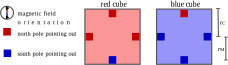
\includegraphics[width=0.75\textwidth]{figures/magnetic_cubes.pdf}
	\caption[Top-down view of the two magnetic modular cube types]{Simplified top-down view of the two magnetic modular cube types with their outward pointing magnet poles, illustrated as red and blue squares. Also visualizes the lengths $r_C$ and $r_M$}
	\label{fig:magnetic_cubes}
\end{figure}

\section{Magnetic Modular Cubes}
The magnetic modular cubes are cube-shaped bodies embedded with permanent magnets on the four side faces.
The magnets have different orientations of their north and south pole. 
One pole is always pointing outside and the other straight to the center of the cube.
The magnet at the front face has its north pole pointing outwards and the magnet at the back its south pole.
These two magnets ensure that the cube is always aligned with the global magnetic field and this orientation holds true for both cube types.
The two other side faces must have the same outwards pointing pole, so that it is not possible for this axis to align with the magnetic field.

In fact, this is the reason a distinct definition of front, back and side is even possible.
Since the front is always pointing to the north pole of the magnetic field, we also call it the north face, or north edge in two dimensions, and all the other faces can also be called by their corresponding cardinal direction.
For each face we define a vector $\vec{e} \in \{ \vec{N},\vec{E},\vec{S},\vec{W}\}$ with $\lVert \vec{e} \rVert = 1$ pointing the the cardinal direction of the magnetic field.
For simplification we call magnets by their outwards pointing pole in further sections.

Furthermore, two different cube types are defined:
Either both side magnets point out their north pole, these cubes are called red cubes, or they point out their south pole, which is then called a blue cube.
\autoref{fig:magnetic_cubes} shows a top-down view of the two cube types with all the outwards pointing magnet poles.
A compass always shows the orientation of the magnetic field in our illustrations.

Magnetic Modular Cubes can be constructed in different sizes and ways. For more technical details and length measurements, we refer to the original \cite{Bhattacharjee2022}.
Two important lengths that we use for planning and simulating are the cube radius $r_C$ and the magnet radius $r_M$ (also illustrated in \autoref{fig:magnetic_cubes}).
$r_C$ is one half-length of a cube face and $r_M$ is the distance from the center of the cube to the center of the magnet.

\begin{figure}
	\centering
	\includegraphics[width=0.53\textwidth]{figures/workspace_config.png}
	\caption[Workspace with a configuration of four magnetic modular cubes]{Rectangular workspace with a configuration of four magnetic modular cubes. All cubes have the same orientation as the magnetic field, indicated by the compass in the top-left corner.}
	\label{fig:workspace_config}
\end{figure}

\section{Workspace and Configuration}
Magnetic modular cubes could theoretical be placed and maneuvered on any 2-dimensional plane with numerous obstacles, as long as you can surround the workspace with a time varying magnetic field.
The magnetic field should be able to point in any direction specified by angles of latitude and longitude, so that the cubes can operate in all desired motion modes.
Because the motion planning problem of self-assembling target shapes in the special Euclidean group is hard enough without considering obstacles and arbitrary workspace shapes, we only work in a rectangular workspace with no internal obstacles.
The workspace is limited by surrounding walls, which are the only objects that could be considered as obstacles in classical motion planning.
However, we do not assume a fixed size, as long as the workspace stays finite and rectangular.

For planning we work in the configuration space of the 2-dimensional special Euclidean group $SE(2) = \mathbb{R}^2 \times \mathbb{S}^1$.
When only considering one cube, the group consists of the position in $\mathbb{R}^2$ and an orientation $\mathbb{S} = [0,2\pi)$ \cite{LaValle2006}.
When working with $n$ cubes, the dimension of our configuration space increases to $\mathbb{R}^{2n} \times \mathbb{S}^1$.
Note that we can still assume only one orientation for $n$ cubes, because we are working with a global magnetic field orienting all cubes the same way.
\autoref{fig:workspace_config} shows a configuration with four cubes in the workspace.
It is irrelevant which exact physical cube is at which position as long as they are the same type, so switching the positions of the two red cubes in \autoref{fig:workspace_config} would lead to the same configuration as before.

\begin{figure}
	\centering
	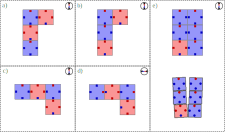
\includegraphics[width=0.65\textwidth]{figures/polyominoes.pdf}
	\caption[Examples of Polyominoes and their equality]{Examples of polyominoes and their equality. a) and d) are equal, only the magnetic field changed its orientation. a) and c) are not equal, they have the same shape but rotated. a) and c) are also not equal because of different cube types in the same shape. e) shows an invalid polyomino in its grid representation (top) and how it behaves in the simulation (bottom).}
	\label{fig:polyominoes}
\end{figure}

\section{Polyominoes}
\label{sec:polys}
The embedded magnets not only align the cube with the magnetic field, they also allow cubes to self-assemble into polyominoes.
Two cube faces can connect if their magnets have opposite polarities.
Because of this and the alignment with the magnetic field, cubes can either be connected at north and south faces, or east and west faces, if the cubes are not the same type.
A polyomino is a set of uniformly sized cubes on a 2-dimensional grid.
Because we work with arbitrary positions and orientations the grid alignment does not hold true for multiple polyominoes in the workspace, but for each polyomino on its own the cubes can be represented in a local coordinate system with position $(x,y)$, $x,y \in \mathbb{Z}$ \cite{Lu2021}.

We consider fixed polyominoes, meaning that two polyominoes are distinct if their shape or orientation are different \cite{Lu2021}.
The magnetic field always provides an orientation, so in \autoref{fig:polyominoes} a) and d) the polyominoes are equal, just the magnetic field is rotated.
Conversely, the polyominoes in \autoref{fig:polyominoes} a) and c) are the same shape but with a different rotation under the same magnetic field orientation, so they are not equal.
Furthermore, two polyominoes are only equal if all the cubes at equal positions are the same type.
The polyominoes in \autoref{fig:polyominoes} a) and b) are not equal because the cube types differ.
It is possible that a workspace contains multiple equal polyominoes.
In that case, we refer to them as being the same polyomino-type, instead of calling them equal, since it is important to differentiate between physical polyominoes with different positions.

The size of a polyomino is the number of cubes it consists of.
Because it is easier to view all structures in the workspace as a polyomino, single cubes are often referred to as trivial polyominoes with size 1.
Although it is not possible to connect cubes of same type at east and west faces, the magnetic modular cubes can assemble structures like the one shown in \autoref{fig:polyominoes} e).
The connection of the bottom two cubes is strong enough to hold the structure together, even though the four blue cubes on the top repel each other.
The resulting polyomino in its grid representation has two east-west connections between cubes the same type and is therefor marked as an invalid polyomino.

\begin{figure}
	\centering
	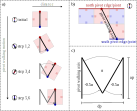
\includegraphics[width=0.80\textwidth]{figures/pivot_walking.pdf}
	\caption[Illustration of the pivot walking motion]{This figure describes the pivot walking motion in detail. a) shows the six pivot walking steps for a single red cube. You can see the orientation of the magnetic field (bigger arrow indicates elevation). In b) an example polyomino with its pivot axis, edges and points is shown. c) illustrates the rotation of the pivot axis labeled with all the pivot walking parameters.}
	\label{fig:pivot_walking}
\end{figure}

\section{Motion Modes}
\label{sec:motion}
In \cite{Bhattacharjee2022} three motion modes are presented. Rotation, pivot walking and rolling.

If the magnetic field orientation lays in the plane of the workspace and rotates without any inclination the rotation is performed around the center of mass for all polyominoes and we consider this motion a normal rotation.

Rotating the magnetic field perpendicular to the workspace plane, cubes can roll forwards or backwards.
This rolling motion becomes problematic for self-assembly, because the top and bottom face of the cube, which contain no magnets, can become a side face.
Because rotation and pivot walking are sufficient to reach any position in the workspace, we do not consider rolling in our simulation and planning algorithms.

When elevating the magnetic field orientation by lifting up the south pole slightly, all polyominoes will pivot on the north face bottom edges of their most north-placed cubes.
Pulling up the north pole does the opposite. The polyominoes will pivot on the south face bottom edges of their most south-placed cubes.
The sum of all these cube edges is called the north or south pivot-edge and by keeping the magnetic field elevated and rotating around the normal vector of the workspace plane, the polyominoes will rotate around the center point of their pivot-edge.
This point is called the north or south pivot-point.
All these edges and points are illustrated in \autoref{fig:pivot_walking} b).

\begin{figure}
	\centering
	\includegraphics[width=0.70\textwidth]{figures/plots/pivot_walking_angle.pdf}
	\caption[Functions of $d_p$ based on $\alpha$ for different $a_p$]{Functions of the pivot walking distance $d_p$ based on pivot walking angle $\alpha$ for different pivot walking axes with length $a_p$. Length are giveen in multiples of cube radius $r_C$.}
	\label{fig:pw_angle_plot}
\end{figure}

\begin{figure}
	\centering
	\includegraphics[width=0.70\textwidth]{figures/displacement_pivot_walking.png}
	\caption[Polyomino shapes with different displacement vectors]{All 19 four-cube polyomino shapes with their displacement vector $\vec{d}$ for one pivot walking cycle with $\alpha = \frac{\pi}{4}$. $\vec{d}$ is drawn from the center of mass (red dot). North and south pivot point are drawn as blue and brown dots.}
	\label{fig:displacement_pivot_walking}
\end{figure}

\paragraph{pivot walking:}
Not rotating around the center of mass is important for pivot walking.
In the first step of a pivot waking cycle, the magnetic field is elevated to let the polyomino pivot on its north pivot edge.
As a second step a rotation of $-\frac{1}{2} \cdot \alpha$ is performed around the north pivot point.
$-\pi \leq \alpha \leq \pi$ is the pivot walking angle.
For step 3 and 4 the elevation changes to its opposite to perform a rotation of $\alpha$ around the south pivot point.
Step 5 and 6 are equal to 1 and 2 and will bring the polyomino back to its original orientation.
You can see the pivot walking cycle steps in \autoref{fig:pivot_walking} a) and have a closer look at its parameters in \autoref{fig:pivot_walking} c).

After one pivot walking cycle, the polyomino has moved by a displacement vector $\vec{d}$ with $\lVert \vec{d} \rVert = d_p$, so $d_p$ is the distance the polyomino moved.
The direction and length of $\vec{d}$ changes with the shape of the polyomino.
The movement is always perpendicular to the pivot walking axis $\vec{a}$ with $\lVert \vec{a} \rVert = a_p$, which is the vector between the north and the south pivot point, visualized in \autoref{fig:pivot_walking} b).
$d_p$ can be calculated as
\begin{equation}
d_p = 2 \cdot \sin\left(\frac{1}{2} \cdot \alpha \right) \cdot a_p \,.
\end{equation}
\autoref{fig:pw_angle_plot} shows functions for this equation based on $\alpha$ for different $a_p$.
To calculate $\vec{d}$ you can take the perpendicular of $\vec{a}$ and scale it to the length $d_p$.

When a big $\alpha$ is chosen according to amount, $d_p$ becomes also bigger, but the polyomino needs more space to the north and south to perform the rotations.
For better maneuvering smaller values of $\alpha$ are preferable.
There is a strong deviation of length and direction of the displacement for different polyomino shapes.
So doing a pivot walking motion might not move two polyominoes in the same direction.
\autoref{fig:displacement_pivot_walking} shows all 19 four-cube polyomino shapes with their displacement vectors.
There are still two options for pivot walking, depending on a negative or positive value of $\alpha$.
You can walk left, in the direction of the west-faces, or right, in the direction of the east-faces.
Although the polyomino actually moves in the direction of $\vec{d}$, we can still say that for instance a pivot walk right moves to the east, because $\left| \angle \left( \vec{E}, \vec{d} \right) \right| < \frac{\pi}{2}$.
We call these two options the pivot walking direction $\vec{w} \in \{\vec{E}, \vec{W}\}$.

	\chapter{Algorithmic Approaches}

In this section, several algorithmic approaches to solving the Polyomino Assembly Problem with and without fixed seed tiles are investigated. First, we discuss the hardness of the investigated problems; subsequently, several algorithms are developed. The main focus is on heuristic search-based algorithms, specifically best-first search with various heuristics. Some of the developed heuristics are admissible, meaning that they never overestimate the distance to the target configuration and thus lead to an A* search, which finds sequences of optimal length as solutions, whereas other approaches give up on optimality in exchange for an improved runtime. Furthermore, during the expansion of the search tree, branches that provably cannot lead to a solution can be pruned in order to avoid unnecessary computations. This means, that the configuration represented by these nodes is never used for later expansion steps. Multiple pruning methods are investigated. In addition to the search-based algorithms, we propose an approach using RRTs. Finally, a method for shortening an existing solution is briefly examined.


\section{Hardness of the Problems}
The PSPACE-completeness of the Polyomino Assembly Problem without fixed seed tile follows directly from the PSPACE-completeness of the occupancy problem. For the Fixed Seed Tile Polyomino Assembly Problem, we show, that it is PSPACE-complete even under the conditions, that there are exactly as many tiles on the board as needed to assemble the target shape and the number of glues is constant.

\begin{theorem}
The Fixed Seed Tile Polyomino Assembly Problem is in PSPACE
\end{theorem}

\begin{proof}
Repeated, non-deterministic selection of control inputs until the target shape is assembled solves the problem and only requires us to store the current configuration. Therefore, the problem is in NPSPACE, which is equal to PSPACE.
\end{proof}

\begin{theorem}
The Fixed Seed Tile Polyomino Assembly Problem is PSPACE-hard
\end{theorem}

\begin{figure}
\centering
\includegraphics[width=\textwidth]{figures/hardnessproof.pdf}
\caption[Reduction of the $k$-region relocation problem to Fixed Seed Tile Polyomino Assembly Problem]{Reduction of the $k$-region relocation problem to the Fixed Seed Tile Polyomino Assembly Problem. The red square is the fixed seed tile, the yellow tile $t_{\text{reloc}}$ needs to be relocated $3$ positions to the right in order to assemble the target shape. The blue squares are other tiles. Figure recreated and adapted from \cite{Caballero2020a}.}
\label{fig:hardnessproof}
\end{figure}

\begin{proof}
To show PSPACE-hardness we adapt a proof from ~\cite{Caballero2020a} and reduce from the \emph{$k$-region relocation problem} of the full-tilt model~\cite{BalanzaMartinez2020}. In this problem, $k$ disjoint regions each contain a single tile. The goal is to move all $k$ tiles to the $1 \times 3$ region at the bottom of their respective component using tilt transformations. Analogous to \cite{Caballero2020a}, we start the reduction by connecting the $1 \times 3$ regions to a single bottom row and invert tile placement by placing tiles on all open spaces that did not contain a tile in the original instance of the $k$-region relocation problem. Additionally, we place a fixed seed tile $k$ positions to the right and $1$ down from the leftmost tile in the bottom row $t_{\text{reloc}}$, as shown in Figure \ref{fig:hardnessproof}. We assign glues as follows: The fixed seed tile has glue $A$ on all four edges. $t_{\text{reloc}}$ has glue $B$ on all edges. Every other tile has glue $C$ on all edges. Furthermore, we define the glue function $G$, such that $G(A,B) = G(B,C) = G(C,C) = 1$ and $G(X, Y) = 0$ for all other pairs of glues $X, Y$. Finally, we define the target shape as all open spaces inside the connected region, except for the $k$ leftmost positions in the bottom row. Now a solution to the constructed instance of the Fixed Seed Tile Polyomino Assembly Problem corresponds to a solution to the original instance of the $k$-region relocation problem. The key idea is, that tiles can only bond if they are connected to the seed tile and that only $t_{\text{reloc}}$ can directly bond with the seed tile according to the glue function. Therefore, $t_{\text{reloc}}$ must be relocated $k$ positions to the right, which was shown to solve the original $k$-region relocation problem (in \cite{Caballero2020a}). Conversely, once $t_{\text{reloc}}$ has been successfully moved $k$ spaces to the right, the target shape is immediately assembled, as all open spaces, except the $k$ leftmost positions in the bottom row, are filled with tiles that can bond according to the glue function and are connected to the fixed seed tile via $t_{\text{reloc}}$.
\end{proof}

\begin{corollary}
The Fixed Seed Tile Polyomino Assembly Problem with extra tiles is PSPACE-hard.
\end{corollary}

Note that this leaves open whether the problem is PSPACE-hard when only a single glue other than the \texttt{null} glue is allowed.

\section {Best-First Search}
We explore two different approaches to best-first search. The first approach aims to build the target polyomino directly by minimizing a function of the distances of tiles to the target shape. The second approach aims to build the target polyomino iteratively by adding one tile after the other, while at the same time attempting to keep the remaining tiles separate. \par
To avoid repeatedly visiting the same configuration, information that allows the identification of previously visited board positions must be stored. In our implementation, we compute and store hash values based on the positions and glues of all tiles in order to uniquely identify configurations on a given board.

\subsection {All Tiles at the Same Time}
As the basis for the following heuristic functions, the concept of the $n$ nearest available tiles is used. \par
Given an instance of the Polyomino Assembly Problem with configuration $C = (B, T)$ and a target shape $X$ with $|X| = n$. Let $T_{\text{available}}$ be the set of tiles which are part of a polyomino $P$ for which a path exists that avoids blocked positions in $B$ and along which $P$ can be moved to a position where it is contained in $X$. Assuming that $|X| \leq |T_{\text{available}}|$, $d$ is the distance of the $n$-th nearest tile to the target shape in $T_{\text{available}}$ and $T^\prime= \{t \in T_{ \text{available}} \mid d(t) \leq d \}$.
The branch can be pruned, if $|T_{\text{available}}|$ contains fewer tiles than needed for the target shape

\paragraph{Greatest Distance Heuristic:}
The Greatest Distance heuristic (GD) is an admissible heuristic that can be used in combination with the A* search algorithm. In the resulting algorithm, the value of the heuristic is added to the distance of the current configuration from the initial configuration, i.e., the number of moves required to get to the current configuration. \par
Given a configuration $C$ and a target shape $X$ the heuristic function $h_{\text{GD}}$ is defined as
\begin{equation}
h_{\text{GD}}(C, X) \coloneqq \max_{t \in T^\prime}{d(t)}.
\end{equation}
It is apparent that the greatest distance among the $n$ nearest tiles is a valid lower bound for the number of required moves because every move can reduce the distance of each tile to the target shape by a maximum of $1$ and at least $n$ tiles must reach the target shape in order to complete the assembly. Furthermore, tiles that cannot be part of the target polyomino because they are part of a polyomino that does not fit into the target shape or does not have an unblocked path to the target shape can be ignored. In order to decide if a given tile is in $T_{\text{available}}$, our implementation remembers for each polyomino if it is able to reach the target shape and fits into the target shape. These functions are only reevaluated whenever the polyomino changes. Since polyominoes are expected to change relatively infrequently, the computational overhead should be limited. \par
A heuristic is called consistent if the estimated distance of a node to the goal is never greater than the estimate for any neighboring node plus the cost of reaching that neighbor. As a consequence, an A* search using a consistent heuristic will find the shortest path to any node when that node is processed for the first time. Since a single step, which has a cost of $1$, applied to a configuration reduces the heuristic value of GD by a maximum of $1$ GD is consistent.
\paragraph{Average Distance Heuristic:}
Similar to GD the Average Distance heuristic (AD) is computed based on the distance of the $n$ nearest tiles that can potentially be part of the target shape. A disadvantage of GD is that it only takes into account the greatest distance among the $n$ nearest available tiles and disregards the distances of the closer tiles, which can cause GD to overestimate moves that bring the most distant tile closer but increase the distance of many other tiles to the target shape. The Average Distance heuristic attempts to also take into account the distance of the closer tiles by using the arithmetic mean.
\begin{equation}
h_{\text{AD}}(C, X) \coloneqq \dfrac {\sum_{t \in T^\prime}{d(t)}} {|T^\prime|}
\end{equation}
Following the same logic as above, $h_{\text{AD}}$ is also a consistent heuristic.

\paragraph{Gready Greatest Distance and Greedy Average Distance Heuristic:}
Both $h_{\text{GD}}$ and $h_{\text{AD}}$ can be used in combination with a greedy best-first search approach by not adding the distance from the initial configuration to the heuristic value. If the heuristics are used in this context, we refer to the resulting algorithms as Gready Greatest Distance (GGD) and Greedy Average Distance (GAD) respectively. The idea of this approach is to give up the optimality of the solution in order to potentially improve the execution speed.

\paragraph{Weighted Sum of Distances Heuristic:}
The Weighted Sum of Distances heuristic (WSD) is a non-admissible heuristic, that is an attempt at a generalization of GGD and GAD. While GGD only takes into account the distance of the most distant tile, in GAD the distances of all $n$ nearest available tiles each have the same impact on the heuristic value. WSD allows adjusting the influence that a tile has on the heuristic value based on its distance to the target shape by introducing an exponent $e \in \left[1,\infty\right)$.
\begin{equation}
h_{\text{WSD}} \coloneqq \sum_{t \in T^\prime}{d(t)^e}
\end{equation}
For $e = 1$ WSD behaves equivalently to GAD, whereas for greater $e$, tiles with a greater distance to the target shape have an increased impact on the heuristic function. For a sufficiently large $e$, the heuristic value is essentially defined by the greatest distance among tiles and WSD behaves similar to GGD.

\paragraph{Pruning methods:}
There are multiple pruning methods that can be used together with the all-tiles-at-the-same-time approach. Firstly, if $|T_{\text{available}}| < n$, the configuration can never lead to a solution.
Furthermore, when it can be shown that there is no subset of existing polyominoes which can exactly cover the target shape, the branch can be pruned.
% In general, however, it is NP-complete to decide whether such a tiling of the target shape exists \cite{} and therefore it is not feasible to compute every time a polyomino changes.
Generally, however, it may not be computationally feasible to decide whether such a tiling of the target shape exists every time a polyomino changes.
In the case where there are exactly as many tiles on the board as needed to form the target shape, we determine if the $k$ largest polyominoes can be packed into the target shape. If this is not possible then the branch can be pruned. In our implementation $k = 3$ is selected.


\paragraph{Alternative Stop Condition:}
When the configuration contains exactly as many tiles as needed for the target polyomino, an alternative stop condition can be utilized, which sometimes gets to a solution after fewer expanded nodes.
If at any point during the heuristic search a configuration $C$ contains a single polyomino $P$ that fits exactly into the target shape and for which a path to the target shapes location exists, the sequence leading to $C$, concatenated with a shortest sequence that moves $P$ from its current location to the location of the target shape is a solution to the problem. The later sequence can be found through a breadth-first search. \par
A solution found in this way is not necessarily of optimal length, even if one of the A* search approaches with a consistent heuristic is used. However, it can only be longer than the optimal solution by at most $d_{max}$ steps, where $d_{max}$ is the greatest distance between any two open positions in $B$.


\subsection{One Tile at a Time}

In contrast to the all-tiles-at-the-same-time approach, the one-tile-at-a-time approach uses multiple consecutive best-first searches in order to add tiles one after another to a polyomino. For that reason, the heuristic function used for each of the separate best-first searches depends on the positions of the subassembly and the single tile that it is trying to combine. For that purpose, an implementation of the one-tile-at-a-time approach first needs to compute a set of tiles that can form the target shape and a building order in which these tiles can be added one at a time to construct the target polyomino. Each best-first search attempts to keep all tiles that are not involved in the current construction step separated from each other by pruning configurations with unwanted subassemblies. Importantly, this approach is not a complete solution to the (Fixed Seed Tile) Polyomino Assembly Problem, since it is not always possible to avoid creating multiple subassemblies even if the initial configuration only consists of trivial polyominoes (see Figure \ref{fig:subassemblies}). Furthermore, a found solution is unlikely to be optimal, even if each construction step consists of an A* search with a consistent heuristic. Nevertheless, this method can be effective in many cases. \par
All the following heuristics are used in combination with an A* search.

\begin{figure}
\centering
\includegraphics[width=0.5\textwidth]{figures/subassemblies.pdf}
\caption[Example of necessary subassemblies]{Example instance that requires multiple subassemblies to assemble the target shape (red-striped area) and thus cannot be solved using the one-tile-at-a-time approach.}
\label{fig:subassemblies}
\end{figure}

\paragraph{Minimum Moves to Polyomino heuristic:}
Given a configuration $C = (B, T)$, a target shape $X$ and a Polyomino $P$, the Minimum Moves to Polyomino (MMP) heuristic provides a lower bound on the number of moves required to move a selected tile $t= (p_t, g_t)$ to a position defined relative to the position of $P$. Let $x$ be the absolute coordinates of the target position in the current configuration. For the purpose of the best-first search, the selected target position is always adjacent to a tile in P. Assuming that the absolute target position does not overlap with an obstacle, the heuristic function is defined as follows:
\begin{equation}
h_{\text{MMP}}(C, X, t, x) \coloneqq \left\lceil \dfrac {d(t, x) - d_{1}(t, x)}{2} \right\rceil+ d_{1} (t, x)
\end{equation}
$h_{\text{MMP}}$ is a lower bound on the number of moves required to move $t$ to the target position relative to $P$.

\begin{proof}
A single step reduces the length of a shortest path from $t$ to the target position by a maximum of $2$ because both $t$ and $P$ each move at most one unit distance. However, a move that reduces the distance by $2$ can never reduce the taxicab distance between $t$ and the target position because both $t$ and $P$ must move during the step in order for the distance to be reduced by $2$. By the definition of the step transformation, both $t$ and $P$ must move $1$ unit in the same direction. Therefore, the taxicab distance remains unchanged.
Furthermore, this implies that a single step can reduce the taxicab distance by a maximum of $1$. In this case, one of the components must be stationary and therefore the length of a shortest path is reduced by at most $1$ too. Therefore, a solution needs to contain at least $d_{1} (t, x)$ moves that reduce the length of a shortest path by $1$. This leaves a distance of at least $d(t, x) - d_{1} (t, x)$, which can be reduced by a maximum of $2$ per step.
\end{proof}


\begin{figure}
\centering
\includegraphics[width=0.4\textwidth]{figures/distance.pdf}
\caption[Example for MMP distance]{An example for the MMP distance calculation. The length of the shortest path between the bottom tile and the target position is $9$. The taxicab distance is $3$. Therefore, at least $(9 - 3) \mathbin{/} 2 + 3 = 6$ steps are needed to combine the tiles in the intended way.}
\label{fig:distance}
\end{figure}

Note that the target position can overlap with an obstacle that the target polyomino is adjacent to. In this case, the length of the shortest path to $x$ is replaced by the length of the shortest path to an adjacent position minus $1$. \par
A disadvantage of this heuristic is that it requires knowledge about the pairwise distance of all open positions on the board. In our implementation, these distances are computed in the beginning through breadth-first searches starting on each open position. This is only feasible for small boards as the calculation is $O(m^3)$ where $m$ is the number of open positions, and the memory is $O(m^2)$.

\paragraph{Minimum Moves to Polyomino and Target heuristic:}
The Minimum Moves to Polyomino and Target heuristic (MMPT) tries to mitigate the requirement to compute pairwise distances. For that purpose, the number of required moves as estimated by MMP is only used for the calculation of the heuristic value if both the current subassembly and the selected tile are within some threshold distance $d_t$ of the target area. We define the target area $A$, as the set of all open positions that the finished target polyomino can cover with any of its tiles after a sequence of steps. The target area can be computed with a breadth-first search. The distance of a position $p$ to the target area is called $d_{\text{A}}(p)$ and defined as the length of a shortest path from $p$ (or the nearest open position that $p$ is adjacent to), to the nearest position in the target area.
If the current target position or the selected tile is not near the target area, the maximum distance of the two components to the target area is used as a basis for the heuristic value instead. In this case, to prioritize configurations where both components are near the target area, we apply a factor $w = |A|$. $w$ is proportional to the size of the target area to account for the greater possible distances within a larger target area.
Alternatively $w$ could be selected as the greatest distance within the target area.
\begin{equation}
h_{\text{MMPT}}(C, X, t, x) \coloneqq
\begin{cases}
h_{\text{MMP}}(C, X, t, x), & \text{if } d_{\text{A}}(p_t) \leq d_t \text{ and } d_{\text{A}}(x) \leq d_t\\
w \cdot \max(d_{\text{A}}(p_t), d_{\text{A}}(x)), & \text{otherwise}
\end{cases}
\end{equation}

This approach has two main advantages over MMP. Firstly, it only requires the computation of pairwise distances within the proximity of the target area. Secondly, MMP does not consider in what position the subassembly is formed in relation to the final position of the target shape. This can lead to the formation of subassemblies in locations from where they cannot reach the target shape anymore. In the MMP approach, such branches get pruned; however, the heuristic function does not actively avoid the creation of subassemblies outside the target area. In contrast, MMPT prioritizes forming subassemblies within the reachable area of the target shape.\par
Note that MMPT is not a consistent heuristic.


\paragraph{Distance to Fixed Position heuristic:}
In the case of a fixed seed tile, a much simpler heuristic can be used as a lower bound on the number of required moves to combine a selected tile with the fixed target polyomino.
Because the target position of the tile is fixed, each move can reduce the length of a shortest path from the tile to the target position by a maximum of $1$.
\begin{equation}
h_{\text{DFP}}(C, X, t, x) \coloneqq d(t, x)
\end{equation}
Additionally, during the computation of the shortest paths to the target position, the positions of tiles contained in the fixed polyomino, as well as neighboring positions that are impassable for the selected tile because of glues on the edges of a fixed tile can be marked as blocked.

\paragraph{Pruning methods:}
All of the one-tile-at-a-time approaches require the same two pruning methods. Firstly, a branch is pruned if its configuration contains an unwanted subassembly. Secondly, a branch is pruned if the correct subassembly is present, but is in a location from where it cannot reach a position where it is contained in the target shape.

\paragraph{Computation of the Building Order:}
To compute an order in which tiles can be added to the polyomino, a tiling of the target shape such that all tiles bond is determined using a brute-force algorithm.
Then a recursive backtracking algorithm that removes tiles from the polyomino one after the other is utilized. If all tiles can be removed from the polyomino in this way the reversed deconstruction order is a \emph{potential} building order. To determine if a tile can be removed two conditions are checked.
\begin{enumerate}
\item Do the remaining tiles form a polyomino that is connected by glues?
\item Does a path exist, along which the selected tile can be moved outside of the rectangular region minimally enclosing the polyomino, without being blocked by other tiles or the glues on their edges? This is determined through a breadth-first search.
\end{enumerate}
This approach is directly inspired by research on the constructibility of polyominoes under tilt transformations \cite{Becker2017}.
If this algorithm does not find a potential building order, it is attempted again with a different tiling of the polyomino until a potential building order is found or all possible tilings have been attempted.
A building order found in this way is not guaranteed to be realizable on the board of the problem instance. If any of the best-first searches during the motion planning process terminate without finding a solution, the solver is restarted with another building order.


\section{RRT}
The basic idea of an RRT search is to select a random configuration from the configuration space and expand the configuration in the current tree that is closest according to some cost-to-go function towards the selected configuration. When designing an RRT-based motion planning algorithm for the Polyomino Assembly Problem, the main challenge is to find a cost-to-go function that is fast to compute and provides a reasonable estimate of the distance between two configurations. \par
Let $C_1 = (B, T_1)$ and $C_2 = (B, T_2)$ be two configurations on the same board. 
As a first approach, we constructed a bipartite graph $G = (U, V, E)$ in which the vertices in $U$ represent the tiles from $T_1$ and the vertices in $V$ the tiles from $T_2$. A vertex in $U$ is connected to each vertex in $V$ that represents a tile with the same glues. The weight of the edge is the distance between the positions of the tiles.

Now the cost-to-go from $C_1$ to $C_2$ is estimated by the weight of the longest edge in a bottleneck matching. A bottleneck matching is a perfect matching that minimizes the length of the longest edge between $U$ and $V$. This is a lower bound on the number of steps needed to transform $C_1$ into $C_2$ because every tile in $C_1$ must be moved to a unique target position that contains a tile with the same glues in $C_2$ and each move can reduce the distance of each tile to its target position by a maximum of $1$.
However, the cost-to-go function needs to be evaluated many times during each expansion step of the RRT, and computing a bottleneck matching may be too expensive. Therefore a cost-to-go function that is quicker to compute was investigated. \par

For two tiles $t_1 = (p_1, g_1) \in T_1$ and $t_2 = (p_2, g_2) \in T_2$ we define
\begin{equation}
d_H(t_1, t_2) \coloneqq
\begin{cases}
d(p_1, p_2) , & \text{if } g_1 = g_2 \\
\infty , & \text{otherwise}
\end{cases}
\end{equation}
Then we define the distance between a tile $t$ and a set of tiles $S$ as $D_H(t, S) \coloneqq \min_{s \in S} d_H(s, t)$.
Note that $D_H(t_1, T_2) < \infty$ for any $t_1 \in T_1$, and vice versa, because both sets of tiles have the same sets of glues. \par

Now the cost-to-go-function between $C_1 = (B, T_1)$ and $C_2 = (B, T_2)$ is defined \mbox{equivalently} to the Hausdorff distance \cite{hausdorff} between the two sets of tiles.
\begin{equation}
D_H(C_1, C_2) \coloneqq \max \{	\max_{t_{1} \in T_{1}} d(t_1, T_2) , \max_{t_{2} \in T_{2}} d(t_2, T_1) \}
\end{equation}

Furthermore, if a polyomino exists in $C_1$ that does not fit into any polyomino of $C_2$ we set the cost-to-go to $\infty$. \par
Since the number of times the cost-to-go function is evaluated in each expansion step grows with the number of nodes in the RRT, we try to further mitigate the computational cost of repeatedly evaluating the cost-to-go function by keeping a sparser tree. This is achieved through a more expensive expansion step, which expands the closest node by multiple steps in the direction of the randomly selected configuration. For that purpose, a greedy best-first search with a limited number of iterations is used to minimize the cost-to-go. \par

A downside of both discussed cost-to-go functions is that they require knowledge about the pairwise distances between positions of the board. A potential solution is to use the taxicab distance instead of the length of a shortest path as the underlying distance metric. However, this would further decrease the accuracy of the estimated distance. \par

To estimate the distance to the goal, i.e., any configuration containing the target shape, a different metric must be used because the order of tiles within the target shape and the position of possible left-over tiles are not known. Therefore we choose the greatest distance among the $n$ nearest available tiles, as defined by the GD approach, as an estimate for the distance to the goal. The RRT nodes are kept in a list ordered by the distance to the goal. We bias the RRT search to expand the closest viable node directly towards the goal in $5\%$ of the expansion steps. For these expansion steps, the GGD approach with a limited number of iterations is used. If the distance from the selected node to the goal cannot be reduced in this way, the node is marked as dead and the next expansion towards the goal will use the next closest node. \par


\section {Solution Shortening}
Given two configurations $C_1$ and $C_2$ in which the tiles have the same positions relative to each other. Using a breadth-first search we can efficiently determine whether a sequence of inputs exists that transforms $C_1$ into $C_2$ and that preserves the relative positions of tiles after every step.
This can be used as a way to shorten a solution found by a motion planner as follows.\par
Start at the first position of the original sequence and find the last configuration that contains the same relative positions of tiles as the current configuration. If a sequence of steps between the two configurations shorter than the original sequence can be found using the above method, replace this part of the solution with the shorter sequence. Continue this process for the rest of the sequence.


	\chapter{Experiments}
In this chapter, the presented algorithmic approaches are experimentally evaluated on sets of procedurally generated instances with different features, including instances of both the problem with and without fixed seed tile. Furthermore, we investigate the impact of several parameters, such as the number of tiles, the size of the board, the placement of obstacles, etc., on the difficulty of the problem. The main focus of the analysis is on the comparison of runtimes and the quality (length) of the found solutions. Additionally, the memory requirements of our implementations and the effectiveness of the proposed solution shortening method are briefly evaluated.

\section{Method for Instance Creation}

\begin{figure}
\centering
\begin{subfigure}[b]{0.45\textwidth}
\centering

\includegraphics[width=\textwidth]{figures/example_boards/cave_example.pdf}
\caption{Example cave board instance}
\label{fig:cave}
\end{subfigure}
\hfill
\begin{subfigure}[b]{0.45\textwidth}
\centering
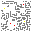
\includegraphics[width=\textwidth]{figures//example_boards/maze_example.pdf}
\caption{Example maze board instance}
\label{fig:maze}
\end{subfigure}
\caption[Example instances for the two different board types]{Example instances for the two different board types. The grey squares represent blocked positions and the colored squares are tiles. The red-striped area marks the target shape. The border is implicitly considered as blocked.}
\label{fig:instance_example}
\end{figure}

To create a sufficient number of instances with a range of different features for experimentation, we implemented a Python function, that procedurally generates such instances based on six input parameters.
\begin{enumerate}
\setlength\itemsep{-0.3em}
\item \textbf{Board type:} This parameter decides which randomized algorithm is used to determine the blocked positions on the board. Two different board types were used for the experiments. The first type is called \emph{maze} and boards of this type are created in a two-step process. Firstly, starting on a board filled with blocked positions, a randomized recursive backtracking algorithm creates a tree of open spaces. Secondly, a number of rectangular open regions proportional to the size of the board is added uniformly at random. The second type is called \emph{cave}. Boards of this type are created using cellular automata, with the following rules: A dead cell becomes alive in the next generation if it has 5 or more living neighbors. A living cell becomes dead in the next generation if it has less than 4 living neighbors. After applying two generations of these rules to a grid where each cell starts alive with a probability of $0.45$, the positions of the living cells correspond to the blocked positions on the cave board. Additionally, to ensure connectedness, the largest connected component of open spaces is determined and all other open spaces are filled. The idea is to create boards with different properties in order to evaluate the influence of obstacle placement on the motion planning algorithms. Maze boards contain open areas, that are connected through narrow corridors; whereas cave boards contain fewer narrow sections.
\item \textbf{Target shape size:}
The number of tiles that are required to assemble the target shape.
\item \textbf{Board size:}
For the experiments, only square-shaped boards were used. The board size determines the edge length of the board.
\item \textbf{Number of extra tiles:}
The number of tiles added to the initial configuration which are not needed to create the target shape. The total number of tiles is the sum of the target shape size and the number of extra tiles.
\item \textbf{Number of glues:}
The number of different glues. The glues on the edges of each tile are selected uniformly at random from the set of available glues. To make it more likely for instances to have a solution, a subset of the tiles is arranged into the target shape and a set of rules is added such that they bond. Finally, additional rules are selected at random, until at least half of all possible combinations of glues stick together.
\item \textbf{Problem type:}
The problem type determines whether a fixed seed tile exists or not. If a fixed seed tile exists, tiles can only bond, if the resulting polyomino contains the fixed tile.
\end{enumerate}

To determine the initial tile positions, tiles are successively placed on legal positions uniformly at random. A position is considered legal, if it is open, does not contain a tile, and is not adjacent to a position containing a tile. The last condition ensures that the initial configuration only contains $1 \times 1$ polyominoes. If a fixed seed tile is required, it is placed first on a suitable position within the target shape. On all generated boards, the open positions form a connected region. Although some measures were taken to increase the probability that the created instances are solvable, instances are not guaranteed to have a solution.

\section{Experimental Setup}
This section explains the methods and tools we used for the experiments and provides an overview of the evaluated algorithmic approaches.

\subsection{Simulation Environment}
For the experiments, all discussed motion planning algorithms were implemented in a self-developed simulator, which is based on TumbleTiles \footnote{TumbleTiles on Github: \url{https://github.com/asarg/TumbleTiles}}. The original TumbleTiles software was upgraded from Python 2 to Python 3 and heavily modified. It is capable of simulating step transformations on configurations with and without fixed seed tile. Furthermore, we implemented support for custom glue functions. Additionally, the software features a GUI that allows the user to view and edit a configuration, animate step sequences, and execute the various motion planning algorithms. \par
The experiments were conducted on multiple computers, each with the same specifications (\textbf{Intel(R) Core(TM) i7-6700K CPU @ 4x4.00GHz, 64GB RAM}) running Ubuntu 20.04 LTS. Multiple motion planning algorithms were evaluated at the same time using different CPU cores.

\subsection{Evaluated Approaches}
This subsection provides an overview of the $10$ evaluated motion planning algorithms and the abbreviations that will be used to refer to them in the following. Furthermore, details about the used parameters are listed if required.
\begin{enumerate}
\setlength\itemsep{0.2em}
\item Breadth-first-search (BFS)
\item Greatest Distance heuristic (GD)
\item Average Distance heuristic (AD)
\item Greedy Greatest Distance heuristic (GGD)
\item Greedy Average Distance heuristic (GAD)
\item Weighted Sum of Distances heuristic (WSD): $e =2$.
\item Minimum Moves to Polyomino heuristic (MMP)
\item Minimum Moves to Polyomino or Target area heuristic (MMPT): $d_t = 4$.
\item Distance to Fixed Position heuristic (DFP)
\item Rapidly-exploring Random Tree (RRT): The Hausdorf-distance based on the shortest path length is used as the cost-to-go function. Each expansion step consists of $40$ iterations of a greedy best-first search. The bias towards the goal is $5$\%. Below a threshold distance of $7$ or less to the goal, a best-first search limited to $500$ iterations attempts to find a solution.
\end{enumerate}

For each solver, all applicable pruning methods discussed in Chapter 3 were used.
Additionally, in combination with the all-tiles-at-the-same-time heuristic approaches (GD, AD, GGD, GAD, WSD) the alternative stop condition from Section 3.2.1 was used, if the configuration contained no extra tiles.

\subsection{Experimental Procedure}
The motion planning algorithms were evaluated on two sets of instances, which were created in advance and contain the same instances for every experiment.

\paragraph{\texttt{InstanceSet1}} consists of relatively easy to solve instances, that allow a comparison of all solvers, including the breadth-first search solver and other (near-)optimal solvers. It contains 5 procedurally generated instances for each possible combination of parameters from the following table.
\begin{center}
\begin{tabular}{ |l|r| }
\hline
Board type & cave, maze \\
\hline
Target shape size & $3 , 4, 5 , 6$ \\
\hline
Board size & $20 , 30, 40$ \\
\hline
Extra tiles & $0, 1, 3$ \\
\hline
Number of glues & $1 , 2, 3$ \\
\hline
Problem type & $\text{seed tile}, \text{no seed tile}$ \\
\hline
% \caption[Possible parameters for \texttt{InstanceSet1}]{The values of parameters used for the creation of the instances in \texttt{InstanceSet1}}

\end{tabular}
\end{center}

\paragraph{\texttt{InstanceSet2}} consists of instances with a wider range of difficulties. It contains 5 procedurally generated instances or each possible combination of parameters from the following table.
\begin{center}
\begin{tabular}{ |l|r| }
\hline
Board type & cave, maze \\
\hline
Target shape size & $5, 10, 13, 15$ \\
\hline
Board size & $40, 80, 120$ \\
\hline
Extra tiles & $0, 3, 5$ \\
\hline
Number of glues & $1, 3, 5$ \\
\hline
Problem type & $\text{seed tile}, \text{no seed tile}$ \\
\hline
\end{tabular}
% \caption[Possible parameters for \texttt{InstanceSet2}]{The values of parameters used for the creation of the instances in \texttt{InstanceSet2}}
\end{center}

\par

Both sets contain a total of $2160$ instances each. The instances from \texttt{InstanceSet1} were attempted to solve with all $10$ evaluated algorithms, whereas only selected solvers (GAD, WSD, MMPT, DFP) were used for \text{InstanceSet2}. DFP was only used on suitable instances, i.e. instances with a fixed seed tile. \par
All experiments were conducted with a timeout of 600 seconds per instance, after which the motion planning algorithm was stopped if it did not find a solution or proved that no solution exists.\par
Along with the problem instance, the solution sequence (if solved), the runtime, and the peak memory usage were recorded. Additionally, the number of nodes in the search tree, or in the case of one-tile-at-a-time algorithms the sum of nodes in all search trees, was recorded.

\begin{figure}[h]
\centering
\includegraphics[width=0.8\textwidth]{figures/example_boards/exampleboards_annotated.pdf}
\caption [Runtime comparison by problem type for GAD] {Six randomly generated instances of different board sizes from \texttt{InstanceSet1}, three cave boards on the left and three maze boards on the right. The yellow squares are tiles and the red-stripped polyominoes are the target shapes. Glues are not shown.}
\label{fig:example_boards}
\end{figure}



\section{Results}

In this section, our algorithmic approaches are evaluated using the experiment results from both sets of instances.

\subsection{Evaluation of \texttt{InstanceSet1}}

The experiment results from \texttt{InstanceSet1} are used to measure the impact of various parameters on the performance of different motion planning algorithms. The relatively small size of the instances allows every solver including the breadth-first search approach and other near-optimal motion planners to solve a large fraction of instances within the timeout of 10 minutes. This provides a baseline for the performance of the other solvers. Additionally, this data is used to evaluate the impact of several configuration parameters on the efficiency of the different motion planning algorithms and to compare the memory requirements of the different approaches as well as the effectiveness of our solution shortening method.

\subsubsection {Performance of breadth-first search}

Figures \ref{fig:bfs_performance1}, \ref{fig:bfs_performance2} show the runtime distribution and the fraction of instances that were successfully solved within the timeout
for instances with a small number of tiles. Note that the performance decreases sharply with an
increased number of tiles. At 3 tiles, more than $70\%$ were successfully solved or shown to have no solution, whereas at 5 tiles less than $10\%$ of instances were finished before the timeout. Only one instance with 9 tiles was successfully solved. The size of the board also had a significant impact on the performance of the solver. Furthermore, a majority of the solved instances were solved long before the timeout. \\
The length of the solutions found by the BFS solver seems to decrease when the number of tiles on the board increases, as shown in Figure \ref{fig:bfs_performance3}. There are two possible reasons for this. Firstly, an increased density of tiles on the board allows shorter solution sequences for target shapes of the same size. Secondly, for a larger number of tiles, the solver only found a solution before the timeout if a relatively short solution existed. \\
In contrast, the solution length significantly increases with increasing board size.
\newpage

\begin{figure}[H]
\centering
\begin{subfigure}[b]{\textwidth}
\centering
\includegraphics[width=\textwidth]{figures/plots/heuristic_solvers_i1/bfs_time_over_tiles.pdf}
\caption{Runtime distributions by number of tiles as box plot. Only successful solutions are shown.}
\label{fig:bfs_time_over_tiles}
\end{subfigure}
\begin{subfigure}[b]{\textwidth}
\centering
\includegraphics[width=\textwidth]{figures/plots/heuristic_solvers_i1/bfs_time_over_board_size.pdf}
\caption{Runtime distributions by board size as box plot. Only successful solutions are shown.}
\label{fig:bfs_fraction_solved_over_board_size}
\end{subfigure}
\caption[Runtime of the BFS motion planner on \texttt{InstanceSet1}] {Runtime of the Breadth-first-search (BFS) motion planner on \texttt{InstanceSet1} by number of tiles and board size. The boxes show upper and lower quartile, the line the median, the whiskers extend to the most extreme value that is within a proportion of 1.5 of the interquartile range. The white dot indicates the arithmetic mean and the other dots outliers.
All experiments were conducted with a 600 seconds timeout per instance, as shown by the dotted red line.}
\label{fig:bfs_performance1}
\end{figure}
\begin{figure}[H]
\begin{subfigure}[b]{\textwidth}
\centering
\includegraphics[width=\textwidth]{figures/plots/heuristic_solvers_i1/bfs_fraction_solved_over_tiles.pdf}
\caption {Fraction of solved instances by number of tiles.}
\label{fig:bfs_fraction_solved_over_tiles}
\end{subfigure}
\begin{subfigure}[b]{\textwidth}
\centering
\includegraphics[width=\textwidth]{figures/plots/heuristic_solvers_i1/bfs_fraction_solved_over_board_size.pdf}
\caption{Fraction of solved instances by board size.}
\label{fig:bfs_fraction_solved_over_board_size}
\end{subfigure}
\caption [Fraction of \texttt{InstanceSet1} solved by the BFS motion planner] {Fraction of instances from \texttt{InstanceSet1} that were solved by the BFS motion planner or for which the solver determined that no solution exists by number of tiles and board size.}
\label{fig:bfs_performance2}
\end{figure}
\begin{figure}[H]
\begin{subfigure}[b]{\textwidth}
\centering
\includegraphics[width=\textwidth]{figures/plots/heuristic_solvers_i1/bfs_solution_length_over_tiles.pdf}
\caption{Distribution of solution length by number of tiles as box plot.}
\label{fig:bfs_solution_length_over_tiles}
\end{subfigure}
\begin{subfigure}[b]{\textwidth}
\centering
\includegraphics[width=\textwidth]{figures/plots/heuristic_solvers_i1/bfs_solution_length_over_board_size.pdf}
\caption{Distribution of solution length by board size as box plot.}
\label{fig:bfs_solution_length_over_board_size}
\end{subfigure}
\caption[Solution lengths for BFS motion planner on \texttt{InstanceSet1}]{Solution length for the BFS motion planner on \texttt{InstanceSet1} by tiles and board size. Only instances for which a solution was found are taken into account.}
\label{fig:bfs_performance3}
\end{figure}


\subsubsection {Comparision of the all-tiles-at-the-same-time search-based motion planning algorithms}


In this subsection, the performance of the BFS solver and the search-based motion planning algorithms GD, AD, GGD, GAD, and WSD are compared. All of these algorithms are best-first searches that try to minimize a function of the distance of multiple tiles to the target shape.\\
As expected, all heuristic searches show a better performance in terms of runtime and success rate than breadth-first search (see Figures \ref{fig:hs_i1_performance1}, \ref{fig:hs_i1_performance2}). The A* searches with consistent heuristic GD and AD take clearly longer to find a solution and have a lower success rate, especially on instances with greater numbers of tiles, than the greedy best-first search approaches. Interestingly, the GD algorithm seems to perform better than the AD algorithm, whereas the greedy algorithms GGD, GAD, and WSD all show a similar performance. All solvers show a clear decrease in success rate with an increasing number of tiles, whereas for the investigated board sizes GAD and WSD show low sensitivity to a change in board size. Overall, the number of tiles seems to have the greatest impact on the performance. \\
The near-optimal motion planning algorithms expectedly produce solutions of roughly the same length as shown in Figure \ref{fig:hs_i1_performance3}. On the other hand, the solution length for the greedy algorithms was much longer on average and they show clear differences in the quality of the found solutions. The solutions found by GAD and WSD are usually shorter than solutions found by GGD. Again, the size of the board seems to have a greater impact than the number of tiles on the length of the found solution.
However, the solution length of GGD seems to be more sensitive to the number of tiles than other approaches. Since the heuristic value of a configuration in GGD only represents the distance of a single tile to the target shape, the distance of a growing number of tiles to the target shape is ignored, when a large number of tiles is present, which may explain this trend.\\
On instances where both AD and GAD found a solution, the solution of the greedy approach was longer than the near-optimal solution of the A* approach by a factor of $2.96$ on average. However, this factor decreases with an increase in board size as the following table indicates. \\

\begin{center}
\begin{tabular}{ |l|r| }
\hline
Board size & $\text{GAD} / \text{AD}$ solution, mean ratio\\
\hline
$20 \times 20$ & $3.24 \pm 3.78$ \\
\hline
$30 \times 30$ & $2.64 \pm 2.31$ \\
\hline
$40 \times 40$ & $2.49 \pm 2.52$ \\
\hline
\end{tabular}
\captionof{table}{Mean ratio of the length of a solution found by GAD and the solution to the same instance found by AD to 3 significant figures $\pm \text{SD}$ for different board sizes.}
\end{center}

\begin{figure}[H]
\centering
\begin{subfigure}[b]{\textwidth}
\centering
\includegraphics[width=\textwidth]{figures/plots/heuristic_solvers_i1/hs_i1_time_over_tiles.pdf}
\caption{Runtime distributions by number of tiles as box plot. Only successful solutions are shown.}
\label{fig:hs_i1_time_over_tiles}
\end{subfigure}
\begin{subfigure}[b]{\textwidth}
\centering
\includegraphics[width=\textwidth]{figures/plots/heuristic_solvers_i1/hs_i1_time_over_board_size.pdf}
\caption{Runtime distributions by board size as box plot. Only successful solutions are shown.}
\label{fig:hs_i1_time_over_board_size}
\end{subfigure}
\caption[Runtime of the search-based heuristic planners on \texttt{InstanceSet1}]{Comparison of the runtime of search-based heuristic motion planning algorithms on \texttt{InstanceSet1} by number of tiles and board size.}
\label{fig:hs_i1_performance1}
\end{figure}
\begin{figure}[H]
\begin{subfigure}[b]{\textwidth}
\centering
\includegraphics[width=\textwidth]{figures/plots/heuristic_solvers_i1/hs_i1_fraction_solved_over_tiles.pdf}
\caption{Fraction of solved instances by number of tiles.}
\label{fig:hs_i1_fraction_solved_over_tiles}
\end{subfigure}
\begin{subfigure}[b]{\textwidth}
\centering
\includegraphics[width=\textwidth]{figures/plots/heuristic_solvers_i1/hs_i1_fraction_solved_over_board_size.pdf}
\caption{Fraction of solved instances by board size.}
\label{fig:hs_i1_fraction_solved_over_board_size}
\end{subfigure}
\caption [Fraction of \texttt{InstanceSet1} solved by the search-based planners] {Fraction of instances from \texttt{InstanceSet1} that were solved by search-based heuristic motion planning algorithms by number of tiles and board size.}
\label{fig:hs_i1_performance2}
\end{figure}
\begin{figure}[H]
\begin{subfigure}[b]{\textwidth}
\centering
\includegraphics[width=\textwidth]{figures/plots/heuristic_solvers_i1/hs_i1_solution_length_over_tiles.pdf}
\caption{Distribution of solution length by number of tiles as box plot.}
\label{fig:hs_i1_solution_length_over_tiles}
\end{subfigure}
\begin{subfigure}[b]{\textwidth}
\centering
\includegraphics[width=\textwidth]{figures/plots/heuristic_solvers_i1/hs_i1_solution_length_over_board_size.pdf}
\caption{Distribution of solution length by board size as box plot.}
\label{fig:hs_i1_solution_length_over_board_size}
\end{subfigure}
\caption[Solution lengths for search-based heuristic planners on \texttt{InstanceSet1}]{Comparison of the solution length of different search-based heuristic motion planning algorithms on \texttt{InstanceSet1} by tiles and board size. Only instances for which a solution was found are taken into account. Outliers are omitted for better readability.}
\label{fig:hs_i1_performance3}
\end{figure}

\newpage

\subsubsection{Effects of the alternative stop condition}

The alternative stop condition that was used only in the absence of extra tiles causes the near-optimal solvers to find solutions that are within the largest possible distance on the board of the optimal solution. In exchange, sometimes a solution can be found after fewer expanded nodes. Figure \ref{fig:moves_to_target} shows the distributions of steps required to move the assembled final polyomino to the target shape. Note that the BFS algorithm on average assembles the polyomino much further away from the target shape position. The heuristics, which are based on the distance of tiles to the target shape, cause configurations with tiles closer to the target shape to be expanded first. Therefore, the target polyomino is more likely to be assembled close to its target position. In contrast, for the BFS solver, it does not matter where on the board the target polyomino is assembled as long as the target shape position is reachable. This suggests, that for the heuristic-based solvers the impact of the alternative stop condition on the solution length was negligible.

\begin{figure}[htpb]
\centering
\includegraphics[width=\textwidth]{figures/plots/heuristic_solvers_i1/hs_i1_moves_to_target_over_board_size.pdf}
\caption[Number of steps after assembly of the final polyomino]{Boxplot comparison of the number of steps needed to move the assembled target polyomino to the target position for different heuristics, grouped by the size of the board. Only the instances where the alternative stop condition was used are shown.}
\label{fig:moves_to_target}
\end{figure}

\vfill
\newpage

\subsubsection{Performance of the remaining motion planning algorithms}

In this subsection, the performance of the remaining approaches, consisting of the one-tile-at-a-time motion planning algorithms (MMP, MMPT, DFP), as well as RRT, will be investigated. For comparison, GAD is included in the plots.
As shown in Figures \ref{fig:i1_performance1}, \ref{fig:i1_performance2} all one-tile-at-a-time algorithms display a better success rate than GAD on instances with a number of tiles greater than 5. The runtime on instances with many tiles is clearly better too. However, the runtime of MMP appears to be particularly sensitive to an increase in board size.
MMPT does not have this downside and shows superior performance to MMP.
In general, the performance of the one-tile-at-a-time approach seems to degrade much slower than the performance of other approaches when the number of tiles is increased.
\\
The DFP motion planner can only be evaluated on instances of the Fixed Seed Tile Polyomino Assembly Problem. It has a high success rate of around $90\%$ on these instances regardless of the number of tiles and the size of the board. Furthermore, a large majority of instances that are solved by DFP are solved in less than 1 second. \\
RRT displays a similar behavior as GAD but its runtime is more sensitive to increased board size. \\
Regarding the solution lengths, shown in Figure \ref{fig:i1_performance3}, the one-tile-at-a-time algorithms usually produce shorter solutions than other approaches. The length of solutions found by RRT are on average shorter and exhibit lower variance than those found by GAD.
None of the solvers demonstrates a large effect of the number of tiles on the solution length. In contrast, an increased board size correlates with an increased solution length for all solvers.


\begin{figure}[htpb]
\centering
\begin{subfigure}[b]{\textwidth}
\centering
\includegraphics[width=\textwidth]{figures/plots/heuristic_solvers_i1/i1_time_over_tiles.pdf}
\caption{Runtime distributions by number of tiles as box plot. Only successful solutions are shown.}
\label{fig:hs_i1_time_over_tiles}
\end{subfigure}
\begin{subfigure}[b]{\textwidth}
\centering
\includegraphics[width=\textwidth]{figures/plots/heuristic_solvers_i1/i1_time_over_board_size.pdf}
\caption{Runtime distributions by board size as box plot. Only successful solutions are shown.}
\label{fig:hs_i1_time_over_board_size}
\end{subfigure}
\caption[Runtime of several planners on \texttt{InstanceSet1}]{Comparison of the runtime of several motion planning algoritms on \texttt{InstanceSet1} by number of tiles and board size. Outliers are omitted.}
\label{fig:i1_performance1}
\end{figure}
\begin{figure}[htpb]
\begin{subfigure}[b]{\textwidth}
\centering
\includegraphics[width=\textwidth]{figures/plots/heuristic_solvers_i1/i1_fraction_solved_over_tiles.pdf}
\caption{Fraction of solved instances by number of tiles.}
\label{fig:i1_fraction_solved_over_tiles}
\end{subfigure}
\begin{subfigure}[b]{\textwidth}
\centering
\includegraphics[width=\textwidth]{figures/plots/heuristic_solvers_i1/i1_fraction_solved_over_board_size.pdf}
\caption{Fraction of solved instances by board size.}
\label{fig:i1_fraction_solved_over_board_size}
\end{subfigure}
\caption [Fraction of \texttt{InstanceSet1} solved by several planners] {Fraction of instances from \texttt{InstanceSet1} that were solved by different motion planning algorithms by number of tiles and board size.}
\label{fig:i1_performance2}
\end{figure}
\begin{figure}[htpb]
\begin{subfigure}[b]{\textwidth}
\centering
\includegraphics[width=\textwidth]{figures/plots/heuristic_solvers_i1/i1_solution_length_over_tiles.pdf}
\caption{Distribution of solution length by number of tiles as box plot.}
\label{fig:i1_solution_length_over_tiles}
\end{subfigure}
\begin{subfigure}[b]{\textwidth}
\centering
\includegraphics[width=\textwidth]{figures/plots/heuristic_solvers_i1/i1_solution_length_over_board_size.pdf}
\caption{Distribution of solution length by board size as box plot.}
\label{fig:i1_solution_length_over_board_size}
\end{subfigure}
\caption[Solution lengths for several planners on \texttt{InstanceSet1}]{Comparison of the solution length of different motion planning algorithms on \texttt{InstanceSet1} by tiles and board size. Only instances for which a solution was found are taken into account.}
\label{fig:i1_performance3}
\end{figure}

\vfill
\newpage

\subsubsection{Comparison of the difficulty of the two problem types}

\texttt{InstanceSet1} contains instances of both the Polyomino Assembly Problem and the Fixed Seed Tile Polyomino Assembly Problem.
We compare the performance of three fundamentally different motion planning approaches for both problems in order to evaluate which problem is harder to solve in practice.
Figures \ref{fig:gad_fixed}, \ref{fig:mmpt_fixed}, \ref{fig:rrt_fixed} show the runtime performance of GAD, MMPT and RRT respectively. All three solvers demonstrate decisively better performance for the problem with a fixed seed tile. For less than 10 tiles, the time needed to solve an instance of the Fixed Seed Tile Polyomino Assembly Problem does not significantly increase when the number of tiles is increased. This is in stark contrast to instances of the Polyomino Assembly Problem where the runtime increases sharply.
Moreover, DFP provides a very efficient and reliable way to solve instances with fixed seed tile.


\begin{figure}[htpb]
\centering
\includegraphics[width=\textwidth]{figures/plots/heuristic_solvers_i1/gad_i1_fixed_time_over_tiles.pdf}
\caption [Runtime comparison by problem type for GAD] {Comparison of the runtime of the Polyomino Assembly Problem with and without fixed seed tile for the GAD solver by number of tiles.}
\label{fig:gad_fixed}
\end{figure}


\begin{figure}[htpb]
\centering
\includegraphics[width=\textwidth]{figures/plots/heuristic_solvers_i1/mmpt_i1_fixed_time_over_tiles.pdf}
\caption[Runtime comparison by problem type for MMPT]{Comparison of the runtime of the Polyomino Assembly Problem with and without fixed seed tile for the MMPT solver by number of tiles.}
\label{fig:mmpt_fixed}
\end{figure}

\begin{figure}[htpb]
\centering
\includegraphics[width=\textwidth]{figures/plots/heuristic_solvers_i1/rrt_i1_fixed_time_over_tiles.pdf}
\caption [Runtime comparison by problem type for RRT] {Comparison of the runtime of the Polyomino Assembly Problem with and without fixed seed tile for the RRT solver by number of tiles.}
\label{fig:rrt_fixed}
\end{figure}

\vfill

\subsubsection{Effect of the board type on the problem difficulty}

To investigate the effect of the obstacle placement, we compare the performance of motion planning algorithms on maze and cave boards (see Figures \ref{fig:i1_gad_maze_cave}, \ref{fig:i1_mmpt_maze_cave}, \ref{fig:i1_rrt_maze_cave}). GAD and RRT both display a similar success rate for both maze and cave boards, whereas MMPT solved slightly more cave boards than maze boards successfully. However, MMPT needed significantly more time for successful solves of cave boards compared to maze boards. This could indicate that, due to the different topography, undesired subassemblies are created more frequently on cave boards than on maze boards, which would cause the MMPT solver to spend more time trying to avoid the creation of subassemblies. Since GAD and RRT allow the creation of multiple subassemblies, they are less affected by this issue. \\
Across all solvers, the solution length on maze boards was higher than on cave boards of the same size, as shown in Figure \ref{fig:maze_vs_cave_solution_length}.
The reason for this could be the greater average pairwise distance between open spaces on maze boards (see Figure \ref{fig:maze_vs_cave_average_distance}).

\begin{figure}[htpb]
\begin{subfigure}[b]{\textwidth}
\centering
\includegraphics[width=\textwidth]{figures/plots/heuristic_solvers_i1/gad_i1_maze_vs_cave_time.pdf}
\caption{Runtime distributions by number of tiles as box plot. Only successful solutions are shown.}
\label{fig:i1_gad_maze_cave_time}
\end{subfigure}
\begin{subfigure}[b]{\textwidth}
\centering
\includegraphics[width=\textwidth]{figures/plots/heuristic_solvers_i1/gad_i1_maze_vs_cave_fraction_solved.pdf}
\caption{Fraction of solved instances by number of tiles.}
\label{fig:i1_gad_maze_cave_fraction_solved}
\end{subfigure}
\caption[Runtime and success rate of GAD on maze and cave boards]{Comparison of the runtimes and success rates of the GAD motion planner on maze and cave boards by number of tiles.}
\label{fig:i1_gad_maze_cave}
\end{figure}

\begin{figure}[htpb]
\begin{subfigure}[b]{\textwidth}
\centering
\includegraphics[width=\textwidth]{figures/plots/heuristic_solvers_i1/mmpt_i1_maze_vs_cave_time.pdf}
\caption{Runtime distributions by number of tiles as box plot.}
\label{fig:i1_mmpt_maze_cave_time}
\end{subfigure}
\begin{subfigure}[b]{\textwidth}
\centering
\includegraphics[width=\textwidth]{figures/plots/heuristic_solvers_i1/mmpt_i1_maze_vs_cave_fraction_solved.pdf}
\caption{Fraction of solved instances by number of tiles.}
\label{fig:i1_mmpt_maze_cave_fraction_solved}
\end{subfigure}
\caption[Runtime and success rate of MMPT on maze and cave boards]{Comparison of the runtimes and success rates of the MMPT motion planner on maze and cave boards by number of tiles.}
\label{fig:i1_mmpt_maze_cave}
\end{figure}

\begin{figure}[htpb]
\begin{subfigure}[b]{\textwidth}
\centering
\includegraphics[width=\textwidth]{figures/plots/heuristic_solvers_i1/rrt_i1_maze_vs_cave_time.pdf}
\caption{Runtime distributions by number of tiles as box plot.}
\label{fig:i1_rrt_maze_cave_time}
\end{subfigure}
\begin{subfigure}[b]{\textwidth}
\centering
\includegraphics[width=\textwidth]{figures/plots/heuristic_solvers_i1/rrt_i1_maze_vs_cave_fraction_solved.pdf}
\caption{Fraction of solved instances by number of tiles.}
\label{fig:i1_rrt_maze_cave_fraction_solved}
\end{subfigure}
\caption[Runtime and success rate of RRT on maze and cave boards] {Comparison of the runtimes and success rates of the RRT motion planner on maze and cave boards by number of tiles.}
\label{fig:i1_rrt_maze_cave}
\end{figure}


\begin{figure}[htpb]
\centering
\includegraphics[width=\textwidth]{figures/plots/heuristic_solvers_i1/maze_vs_cave_solution_length.pdf}
\caption[Solution length by board type]{Length of found solutions compared for maze and cave boards across all solvers by board size.}
\label{fig:maze_vs_cave_solution_length}
\end{figure}

\begin{figure}[htpb]
\centering
\includegraphics[width=\textwidth]{figures/plots/average_distance_cave_vs_maze.pdf}
\caption[Average pairwise distance on maze and cave boards]{The arithmetic mean of the pairwise distances between two open positions on procedurally generated maze and cave boards of different sizes.}
\label{fig:maze_vs_cave_average_distance}
\end{figure}

\vfill
\newpage

\subsubsection{Effect of the number of unique glues on the problem difficulty}

Figures \ref{fig:i1_gad_glue_types}, \ref{fig:mmpt_i1_glue_types}, \ref{fig:rrt_i1_glue_types} show the influence of different numbers of glue types on the distribution of runtimes and the success rate of GAD, MMPT and RRT. For all solvers, the runtime increases with an increase in the number of glue types. However, MMPT seems to be affected less by an increase in the number of tiles. Moreover, the success rate of MMPT does not decrease with an increased number of glues types. A reason for this is that once the building order of the polyomino is computed, which can be done quickly for the small sizes of target shapes in \texttt{InstanceSet1}, the performance of MMPT is no longer negatively influenced by a high number of glue types. On the contrary, a greater number of glue types causes tiles to create fewer undesired subassemblies.

\begin{figure}[htpb]
\centering
\begin{subfigure}[b]{0.48\textwidth}
\centering
\includegraphics[width=\textwidth]{figures/plots/heuristic_solvers_i1/gad_i1_time_over_glue_types.pdf}
\caption{Runtime distributions by number of tiles as box plot.}
\label{fig:gad_i1_time_over_glue_types}
\end{subfigure}
\hfill
\begin{subfigure}[b]{0.48\textwidth}
\centering
\includegraphics[width=\textwidth]{figures/plots/heuristic_solvers_i1/gad_i1_fraction_solved_over_glue_types.pdf}
\caption{Fraction of solved instances by number of tiles.}
\label{fig:gad_i1_fraction_solved_over_glue_types}
\end{subfigure}
\caption[Runtime and success rate of GAD by number of glue types] {Comparison of the runtime and success rate of the GAD motion planning algorithm by the number of unique glue types.}
\label{fig:i1_gad_glue_types}
\end{figure}

\begin{figure}[htpb]
\centering
\begin{subfigure}[b]{0.48\textwidth}
\centering
\includegraphics[width=\textwidth]{figures/plots/heuristic_solvers_i1/mmpt_i1_time_over_glue_types.pdf}
\caption{Runtime distributions by number of tiles as box plot.}
\label{fig:mmpt_i1_time_over_glue_types}
\end{subfigure}
\hfill
\begin{subfigure}[b]{0.48\textwidth}
\centering
\includegraphics[width=\textwidth]{figures/plots/heuristic_solvers_i1/mmpt_i1_fraction_solved_over_glue_types.pdf}
\caption{Fraction of solved instances by number of tiles.}
\label{fig:mmpt_i1_fraction_solved_over_glue_types}
\end{subfigure}
\caption[Runtime and success rate of MMPT by number of glue types] {Comparison of the runtime and success rate of the MMPT motion planning algorithm by the number of unique glue types.}
\label{fig:mmpt_i1_glue_types}
\end{figure}

\begin{figure}[htpb]
\centering
\begin{subfigure}[b]{0.48\textwidth}
\centering
\includegraphics[width=\textwidth]{figures/plots/heuristic_solvers_i1/rrt_i1_time_over_glue_types.pdf}
\caption{Runtime distributions by number of tiles as box plot.}
\label{fig:rrt_i1_time_over_glue_types}
\end{subfigure}
\hfill
\begin{subfigure}[b]{0.48\textwidth}
\centering
\includegraphics[width=\textwidth]{figures/plots/heuristic_solvers_i1/rrt_i1_fraction_solved_over_glue_types.pdf}
\caption{Fraction of solved instances by number of tiles.}
\label{fig:rrt_i1_fraction_solved_over_glue_types}
\end{subfigure}
\caption[Runtime and success rate of RRT by number of glue types] {Comparison of the runtime and success rate of the RRT motion planning algorithm by the number of unique glue types.}
\label{fig:rrt_i1_glue_types}
\end{figure}

\vfill

\subsubsection{Memory usage}

Aside from the runtime and solution length, it is also interesting to compare the peak memory requirements of the different motion planning approaches.
The peak memory requirement of three motion planning algorithms depending on the time needed to solve an instance are shown in Figures \ref{fig:gad_i1_peek_memory_usage_over_time}, \ref{fig:mmpt_i1_peek_memory_usage_over_time}, \ref{fig:rrt_i1_peek_memory_usage_over_time}.
For GAD and MMPT, the maximum of the peak memory usages implies a linear growth over time, because the speed at which nodes are expanded remains constant over time and the memory requirements per node remain constant. The memory usages of both algorithms cover a similar range with a maximum of around $8$GB and $9$GB respectively.
In contrast, the peak memory usage of RRT is two orders of magnitude smaller, because only a sparse tree of configurations is stored. Furthermore, it does not increase linearly over time. Instead, it increases sharply in the first few seconds and then slows down significantly. An explanation for this behavior is that every iteration requires the computation of the Hausdorf distance from a random configuration to all configurations in the RRT. As the number of nodes grows over time, each iteration takes more time than the previous one. Furthermore, up to a certain number of iterations the memory requirements for a single expansion step, which includes a heuristic search, outweigh the memory requirements of the RRT.

\begin{figure}[htpb]
\centering
\includegraphics[width=\textwidth]{figures/plots/heuristic_solvers_i1/gad_i1_peek_memory_usage_over_time.pdf}
\caption[Memory usage of GAD]{Peak memory usage of GAD in MB depending on the runtime of the solver as scatter plot.}
\label{fig:gad_i1_peek_memory_usage_over_time}
\end{figure}

\begin{figure}[htpb]
\centering
\includegraphics[width=\textwidth]{figures/plots/heuristic_solvers_i1/mmpt_i1_peek_memory_usage_over_time.pdf}
\caption[Memory usage of MMPT]{Peak memory usage of MMPT in MB depending on the runtime of the solver as scatter plot.}
\label{fig:mmpt_i1_peek_memory_usage_over_time}
\end{figure}

\begin{figure}[htpb]
\centering
\includegraphics[width=\textwidth]{figures/plots/heuristic_solvers_i1/rrt_i1_peek_memory_usage_over_time.pdf}
\caption[Memory usage of RRT]{Peak memory usage of RRT in MB depending on the runtime of the solver as scatter plot.}
\label{fig:rrt_i1_peek_memory_usage_over_time}
\end{figure}

\vfill

\subsubsection{Effectiveness of solution shortening methods}

In this subsection, we evaluate the effectiveness of the solution shortening method discussed in Subsection 3.4. \\
We found this method to be most effective for solutions computed with the RRT algorithm (see Figure \ref{fig:solution_shortening}).
Because of the randomized nature of the RRT, it often contains redundant steps that can be removed. The average percentage by which a solution to an instance from \texttt{InstanceSet1} could be shortened in this way is $4.83\%$. This includes only the instances without a fixed seed tile, for which we implemented the method.\\
Sometimes a significant portion of a sequence could be removed. For example, one sequence computed by GGD was shortened from 62 to 36 steps. \\

\begin{figure}[H]
\centering
\includegraphics[width=\textwidth]{figures/plots/heuristic_solvers_i1/solution_shortening.pdf}
\caption[Effectiveness of the solution shortening method]{Length of shortened solutions devided by the length of the original solution for different solvers as box plot. The data consists of the results for instances without fixed seed tiles from \texttt{InstanceSet1}.}
\label{fig:solution_shortening}
\end{figure}

\subsection{Evaluation of \texttt{InstanceSet2}}
In this subsection, we evaluate selected motion planning algorithms that demonstrated a good performance in the previous experiments, on instances with a wider range of parameters.
The results from \texttt{InstanceSet1} show that the near-optimal motion planning algorithms are usually unable to solve larger instances. With regards to the RRT solver, the calculation of the cost-to-go function based on the length of a shortest path is computationally infeasible for the larger boards in \texttt{InstanceSet2}. Therefore, we choose to compare GAD, WSD, MMPT, and DFP.

\subsubsection{Comparison of the motion planning algorithms}

The time needed by the motion planning algorithms and their success rate can be seen in Figures \ref{fig:i2_performance1}, \ref{fig:i2_performance2}. This time the plots are grouped by the target shape size, instead of the total number of tiles on the board. Instances can have up to $5$ additional tiles that are not needed to build the target shape. Generally speaking, the runtime of all algorithms increases with an increased size of the target shape. Again, all algorithms finish a majority of the solved instances long before the timeout, which indicates that there are certain instances that the solvers struggle with, whereas other instances can be solved easily.
The performance of GAD and WSD in terms of the fraction of solved instances continues to decrease sharply with an increase in the size of the target shape. MMPT shows an overall higher success rate but the performance also falls off when the target shape gets is bigger. DFP performs best and shows a high success rate that only declines slowly with an increase in the target shape size and does not fall under $60\%$. Even when the success rate of all solvers is compared exclusively on instances with a fixed seed tile, DFP still has a far higher success rate than the other algorithms, as shown in Figure \ref{fig:i2_fraction_solved_over_target_size_fixed_only}. Furthermore, DFP finds a solution much faster than all other algorithms. Since instances are not guaranteed to have a solution, it is possible that randomly generated instances with a larger target shape are less likely to be solvable, which could also be a factor for the fraction of solved instances.
The greater range of board sizes in \texttt{InstanceSet2} confirms that the runtime increases much faster with an increased number of tiles, rather than increased board size. In particular, the success rate of DFP is not decreased when the board size is increased from $40 \times 40$ to $120 \times 120$. \par
Although the one-tile-at-a-time algorithms solve a larger fraction of instances within the timeout, GAD and WSD can sometimes find solutions faster than MMPT or find solutions to instances that MMPT is not able to solve because MMPT is incomplete. Particularly instances with simple glues and without extra tiles that the one-tile-at-a-time approach could not solve were sometimes efficiently solved by the all-tiles-at-the-same-time approach, as shown in Figure \ref{fig:i2_gad_vs_mmpt}.\par
The solution lengths shown in Figure \ref{fig:i2_performance3} grow with both the size of the board and target shape. The length of solutions found by GAD and WSD seems to be particularly sensitive to an increased target shape size. In comparison, WSD produced slightly shorter sequences than GAD. Overall the one-tile-at-a-time algorithms find shorter solutions than the all-tiles-at-the-same-time algorithms. \\
Note that due to the method through which the instances were created it was relatively easy for the one-tile-at-a-time algorithms to find a valid set of tiles and an order in which a given polyomino can be built because a majority of glue types was guaranteed to stick together. However, for larger target shapes or sparser glue functions, this becomes a challenging task that could limit the efficiency of the one-tile-at-a-time approach.


\begin{figure}[htpb]
\centering
\begin{subfigure}[b]{\textwidth}
\centering
\includegraphics[width=\textwidth]{figures/plots/heuristic_solvers_i2/i2_time_over_target_size.pdf}
\caption{Runtime distributions by target shape size as box plot. Only successful solutions are shown.}
\label{fig:i2_time_over_target_size}
\end{subfigure}
\begin{subfigure}[b]{\textwidth}
\centering
\includegraphics[width=\textwidth]{figures/plots/heuristic_solvers_i2/i2_time_over_board_size.pdf}
\caption{Runtime distributions by board size as box plot. Only successful solutions are shown.}
\label{fig:i2_time_over_board_size}
\end{subfigure}
\caption[Runtime of several motion planners on \texttt{InstanceSet2}]{Comparison of the runtime of four motion planning algoritms on \texttt{InstanceSet2} by target shape size and board size.}
\label{fig:i2_performance1}
\end{figure}
\begin{figure}[htpb]
\begin{subfigure}[b]{\textwidth}
\centering
\includegraphics[width=\textwidth]{figures/plots/heuristic_solvers_i2/i2_fraction_solved_over_target_size.pdf}
\caption{Fraction of solved instances by target shape size.}
\label{fig:i2_fraction_solved_over_target_size}
\end{subfigure}
\begin{subfigure}[b]{\textwidth}
\centering
\includegraphics[width=\textwidth]{figures/plots/heuristic_solvers_i2/i2_fraction_solved_over_board_size.pdf}
\caption{Fraction of solved instances by board size.}
\label{fig:i2_fraction_solved_over_board_size}
\end{subfigure}
\caption [Fraction of \texttt{InstanceSet2} solved by several planners] {Fraction of instances from \texttt{InstanceSet2} that where solved by four motion planning algorithms by target shape size and board size. For DFP the fraction of suitable instances with a fixed tile that were solved is shown.}
\label{fig:i2_performance2}
\end{figure}
\begin{figure}[htpb]
\begin{subfigure}[b]{\textwidth}
\centering
\includegraphics[width=\textwidth]{figures/plots/heuristic_solvers_i2/i2_solution_length_over_target_size.pdf}
\caption{Distribution of solution length by target shape size as box plot.}
\label{fig:i2_solution_length_over_tiles}
\end{subfigure}
\begin{subfigure}[b]{\textwidth}
\centering
\includegraphics[width=\textwidth]{figures/plots/heuristic_solvers_i2/i2_solution_length_over_board_size.pdf}
\caption{Distribution of solution length by board size as box plot.}
\label{fig:i2_solution_length_over_board_size}
\end{subfigure}
\caption[Solution lengths for several planners on \texttt{InstanceSet2}]{Comparison of the solution length of four motion planning algorithms on \texttt{InstanceSet2} by target shape size and board size. Only instances for which a solution was found are taken into account.}
\label{fig:i2_performance3}
\end{figure}

\begin{figure}[htpb]
\centering
\includegraphics[width=\textwidth]{figures/plots/heuristic_solvers_i2/i2_fraction_solved_over_target_size_fixed_only.pdf}
\caption[Fraction of \texttt{InstanceSet2} with fixed tile solved by several planners]{Fraction of instances \textbf{with fixed seed tiles} from \texttt{InstanceSet2} that were solved by four motion planning algorithms by target shape size and board size.}
\label{fig:i2_fraction_solved_over_target_size_fixed_only}
\end{figure}


\begin{figure}[htpb]
\centering
\begin{subfigure}[b]{0.48\textwidth}
\centering
\includegraphics[width=\textwidth]{figures/plots/heuristic_solvers_i2/gad_vs_mmpt_time.pdf}
\caption{Runtime distributions by number of tiles as box plot.}
\label{fig:i2_gad_vs_mmpt_time}
\end{subfigure}
\hfill
\begin{subfigure}[b]{0.48\textwidth}
\centering
\includegraphics[width=\textwidth]{figures/plots/heuristic_solvers_i2/gad_vs_mmpt_fraction_solved.pdf}
\caption{Fraction of solved instances by number of tiles.}
\label{fig:i2_gad_vs_mmpt_rate}
\end{subfigure}
\caption[Runtime and success rate comparison of GAD and WSD] {Comparison of the runtime and success rate of GAD and MMPT on instances from \texttt{InstanceSet2} with exactly one glue and no extra tiles.}
\label{fig:i2_gad_vs_mmpt}
\end{figure}


\vfill

\subsubsection{Effect of extra tiles on the problem difficulty}

In this subsection, the effect of extra tiles that are not needed to assemble the target polyomino on the performance of motion planning algorithms is investigated.
As an example, the runtime and success rate of different solvers depending on the number of extra tiles for the instances from \texttt{InstanceSet2} that have a target shape of size 10 is shown in Figure \ref{fig:i2_extra_tiles_performance}. The negative effect of extra tiles on the success rate seems to be much stronger for GAD and WSD than for other solvers. The reason for this is that GAD and WSD only minimize the distance of the $n$ nearest tiles to the target shape, where $n$ is the target shape size. Hence, whenever it is impossible to build the target shape from the $n$ tiles with the nearest starting positions, this approach is very inefficient. In contrast, DFP only shows a minor decrease in success rate when extra tiles are present.
The results for the runtime of GAD and WSD are not meaningful due to the small fractions of solved instances with extra tiles. MMPT on the other hand displays an increased runtime when a small number of extra tiles are added. Presumably, the greater density of tiles on the board makes it more difficult to avoid undesired subassemblies.\\
Figure \ref{fig:i2_extra_tiles_solution_length} shows that the solution length does not grow when a small number of extra tiles is present. The solution lengths of GAD and WSD appear to be shorter when extra tiles are added, which can be explained by the fact that on average a greater number of tiles start close to the target shape in this case.


\begin{figure}[htpb]
\begin{subfigure}[b]{\textwidth}
\centering
\includegraphics[width=\textwidth]{figures/plots/heuristic_solvers_i2/time_over_extra_tiles.pdf}
\caption{Distribution of runtime by number of extra tiles as box plot. Only successful solutions are shown.}
\label{fig:time_over_extra_tiles}
\end{subfigure}
\begin{subfigure}[b]{\textwidth}
\centering
\includegraphics[width=\textwidth]{figures/plots/heuristic_solvers_i2/fraction_solved_over_extra_tiles.pdf}
\caption{Fraction of solved instances by number of extra tiles.}
\label{fig:i1_extra_tiles_fraction_solved.pdf}
\end{subfigure}
\caption[Runtime and success rate of planners by number of extra tiles] {Comparison of the runtimes and success rates of four motion panning algorithms by the number of extra tiles. Evaluated on the instances from \texttt{InstanceSet2} that have a target shape size of exactly 10.}
\label{fig:i2_extra_tiles_performance}
\end{figure}

\begin{figure}[htpb]
\centering
\includegraphics[width=\textwidth]{figures/plots/heuristic_solvers_i2/solution_length_over_extra_tiles.pdf}
\caption[Solution length of several planners by number of extra tiles] {Comparison of the solution length of four motion panning algorithms by the number of extra tiles. Evaluated on the instances from \texttt{InstanceSet2} that have a target shape size of exactly 10.}
\label{fig:i2_extra_tiles_solution_length}
\end{figure}

	\chapter{Conclusion and Future Work}
In this thesis, we designed motion planning algorithms for the assembly of shapes in the Tilt model based on multiple different approaches, including search-based and sampling-based motion planning algorithms. We evaluated the effectiveness of these approaches experimentally on procedurally created boards and investigated the parameters that are most significant for the performance of motion planning algorithms in general, as well as the specific strength and weaknesses of the different approaches.
We found that the number of tiles on the board has the most significant impact on the runtime, which is an expected result since the difficulty of motion planning problems is known to largely depend on the dimensionality of the configuration space, which is proportional to the number of tiles in the case of Tilt.\par
Our first approach, an A* search in combination with a consistent heuristic based on the distance of tiles to the target shape, is able to find optimal solutions for small numbers of tiles, but quickly becomes computationally infeasible.\par
Greedy best-first search with heuristics based on the distances of tiles to the target shape is more efficient, however it often produces a solution with far from optimal length. On a positive note, the average factor by which a solution found by GAD was longer than a solution to the same instance found by AD was less than 3 for the evaluated instances and seems to decrease for larger boards. Unfortunately, the runtime of greedy best-first search increases sharply when the number of tiles is greater than 10 and is very sensitive to additional tiles that are not needed to construct the target shape, due to the heuristics indifference towards the glue types of tiles and their possible positions within the target shape.
The three proposed greedy best-first search algorithms GGD, GAD, and WSD (with the exponent 2), which all use a heuristic based on the distance of tiles to the target shape, exhibit very similar performance. However, GGD seems to perform worse than the other algorithms as the number of tiles grows and WSD produced solutions of slightly shorter length. Overall, WSD seems to present the best tradeoff between solution length and runtime, which might be further improved by selecting a different exponent.\par
Avoiding subassemblies and adding one tile at a time to the target polyomino can often quickly yield a solution even on boards with more than 10 tiles. However, this approach is not a complete algorithm. Furthermore, it struggles with boards that are densely populated with tiles as well as boards containing few obstacles that separate tiles from each other, because in these cases it becomes hard or even impossible to avoid subassemblies. Another problem for one-tile-at-a-time motion planning algorithms is the necessity to compute a valid construction order for the target shape with regard to the glues on the edges of the available tiles. For complicated glues and large target shapes, this is a hard problem to solve. While a large number of glue types increases the difficulty of assembling the target shape, it helps to avoid the accidental creation of undesired subassemblies and can therefore be advantageous for one-tile-at-a-time algorithms, once they found a valid building order. Whereas for the other evaluated classes of algorithms, more glue types had a negative effect on the performance. \par
A simple solution shortening technique can help to decrease the length of solutions found by non-optimal algorithms and is particularly effective for solutions found with the RRT algorithm. \par
Even though the Fixed Seed Tile Polyomino Assembly Problem is PSPACE-complete, it was much easier to solve at the same numbers of tiles than its counterpart without fixed seed tiles. DFP is a simple and fast motion planning algorithm for this problem, however, it is not complete. In the experiments, DFP solved a large fraction of instances including instances with larger numbers of tiles in a short time. \par
The evaluation of computational complexity for the Polyomino Assembly Problem without a fixed seed tile and without extra tiles is left to future research. \par
RRT is a promising method to solve Tilt motion planning problems. Combined with a computationally more expensive expansion step, it has the added benefit of requiring less memory than other approaches. A major challenge in this context is to find a cost-to-go function that is fast to compute and gives a good approximation of the actual distance between two configurations. Furthermore, the RRT algorithm we designed has a large number of adjustable parameters. Future work could find optimal settings for these parameters and evaluate the effectiveness of other cost-to-go functions. \par
Better best-first search algorithms could potentially be achieved with heuristics that not only depend on the distance of tiles to the target shape but instead consider, for example, the involved glue types and possible positions of tiles within the target polyomino. \par
Another possible direction for future work is to evaluate motion planning algorithms on configurations with parameters outside the scope of this thesis, such as boards that contain a high density of tiles or a small number of obstacles.
	
	\bibliographystyle{abbrv}
	\bibliography{bibliography.bib}

\end{document}